\thispagestyle{foliage-header}
\poemtitle{Hark! The Herald Angels Sing}
\begin{multicols}{2}
\begin{verse}
Hark! the herald angels sing\\
Glory to the newborn King\\
Peace on earth, and mercy mild\\
God and sinners reconciled\\
Joyful, all ye nations, rise\\
Join the triumph of the skies\\
With th' angelic host proclaim\\
Christ is born in Bethlehem\\
Hark, the herald angels sing\\
Glory to the newborn King\\!
\vfill*{}

Hail, the heav'n-born Prince of peace\\*
Hail! the Son of Righteousness\\*
Light and life to all he brings\\*
Risen with healing in his wings\\*
Mild he lays his glory by\\*
Born that man no more may die\\*
Born to raise the some of earth\\*
Born to give them second birth\\*
Hark! the herald angels sing\\*
Glory to the newborn King\\!

Hark, the herald angels sing,\\
Glory to the newborn King\\
Peace on earth, and mercy mild\\
God and sinners reconciled\\
Joyful, all ye nations, rise\\
Join the triumph of the skies\\
With th' angelic host proclaim\\
Christ is born in Bethlehem\\
Hark, the herald angels sing\\
Glory to the newborn King\\!
\end{verse}
\end{multicols}
\begin{tikzpicture}[remember picture,overlay]
\draw  let \p1=($(current page.south)-(current page footer area.north)$),
\n1={veclen(\x1,\y1)} in
node [inner sep=0,outer sep=0,above right] 
at ([xshift=-2.5cm]current page.south west){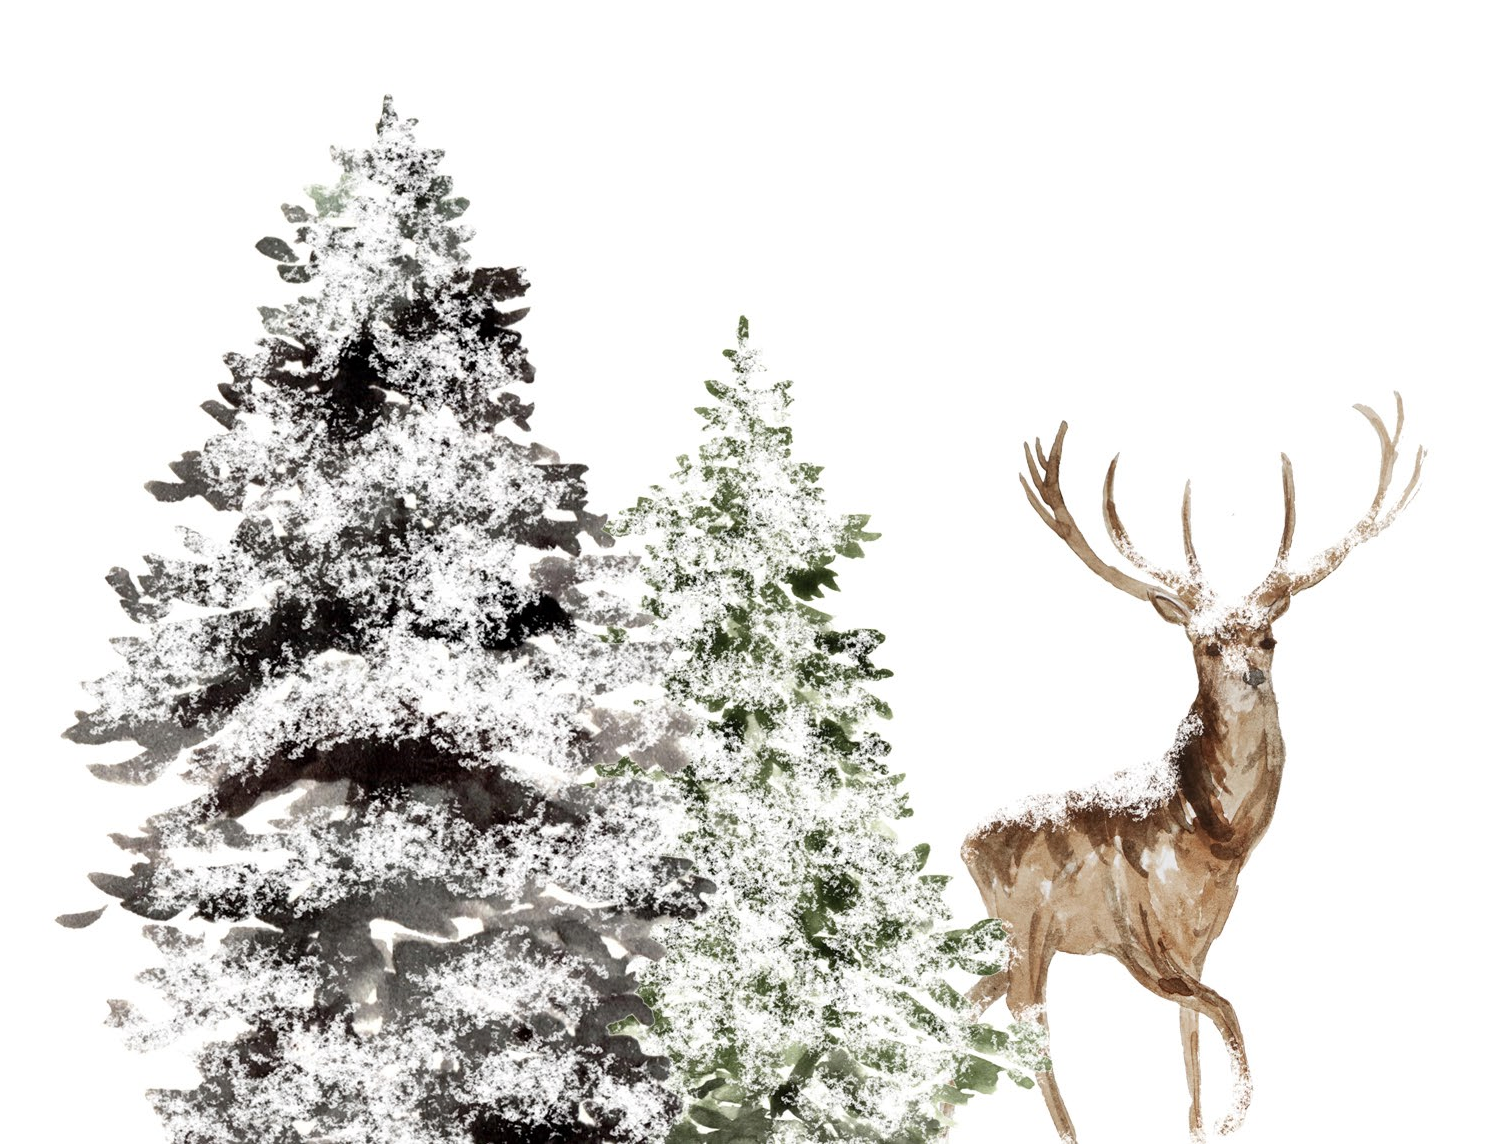
\includegraphics[width=0.7\paperwidth]{images/deer-2}};
\end{tikzpicture}
\pagebreak
